\chapter{Results and Discussion}\label{ch:results_discussion}
This chapter presents the results of our experiments as performed according to the description in Chapter~\ref{ch:methods}. We then discuss our results and conclude the chapter with a comparison of our results in relation to real-world organisms, as well as potential limitations.

\section{Results}\label{results}
In this section we present the results of our experiments. We begin by presenting the results of our statistical analysis before moving on to show the results in various plots. It is of minor note that in many of the figures, a rolling window was used to smooth the values, resulting in many of the plots only showing data starting after a few thousand generations (often 10,000). It should be noted, however, that organisms were evolved for 500,000 generations and that the data is complete. 

\subsection{Statistical Analysis}
Below in Table~ we see the results of our p-value calculations for testing whether the results are significant.   

\subsection{Genome Size}\label{sec:genome_size}
In this section we will examine the results of the different conditions, focusing on which, if any, lead to a reduced genome. Figure~\ref{fig:genome_size}
presents the main findings regarding genome size. In the figure, the blue line represents the control condition and the other colors show the changed conditions: mutation up/down, selection up/down, and population up/down. As can be seen from the figure,the results did not actually vary all that much across the conditions with regard to genome size.  
\begin{figure}[H]
	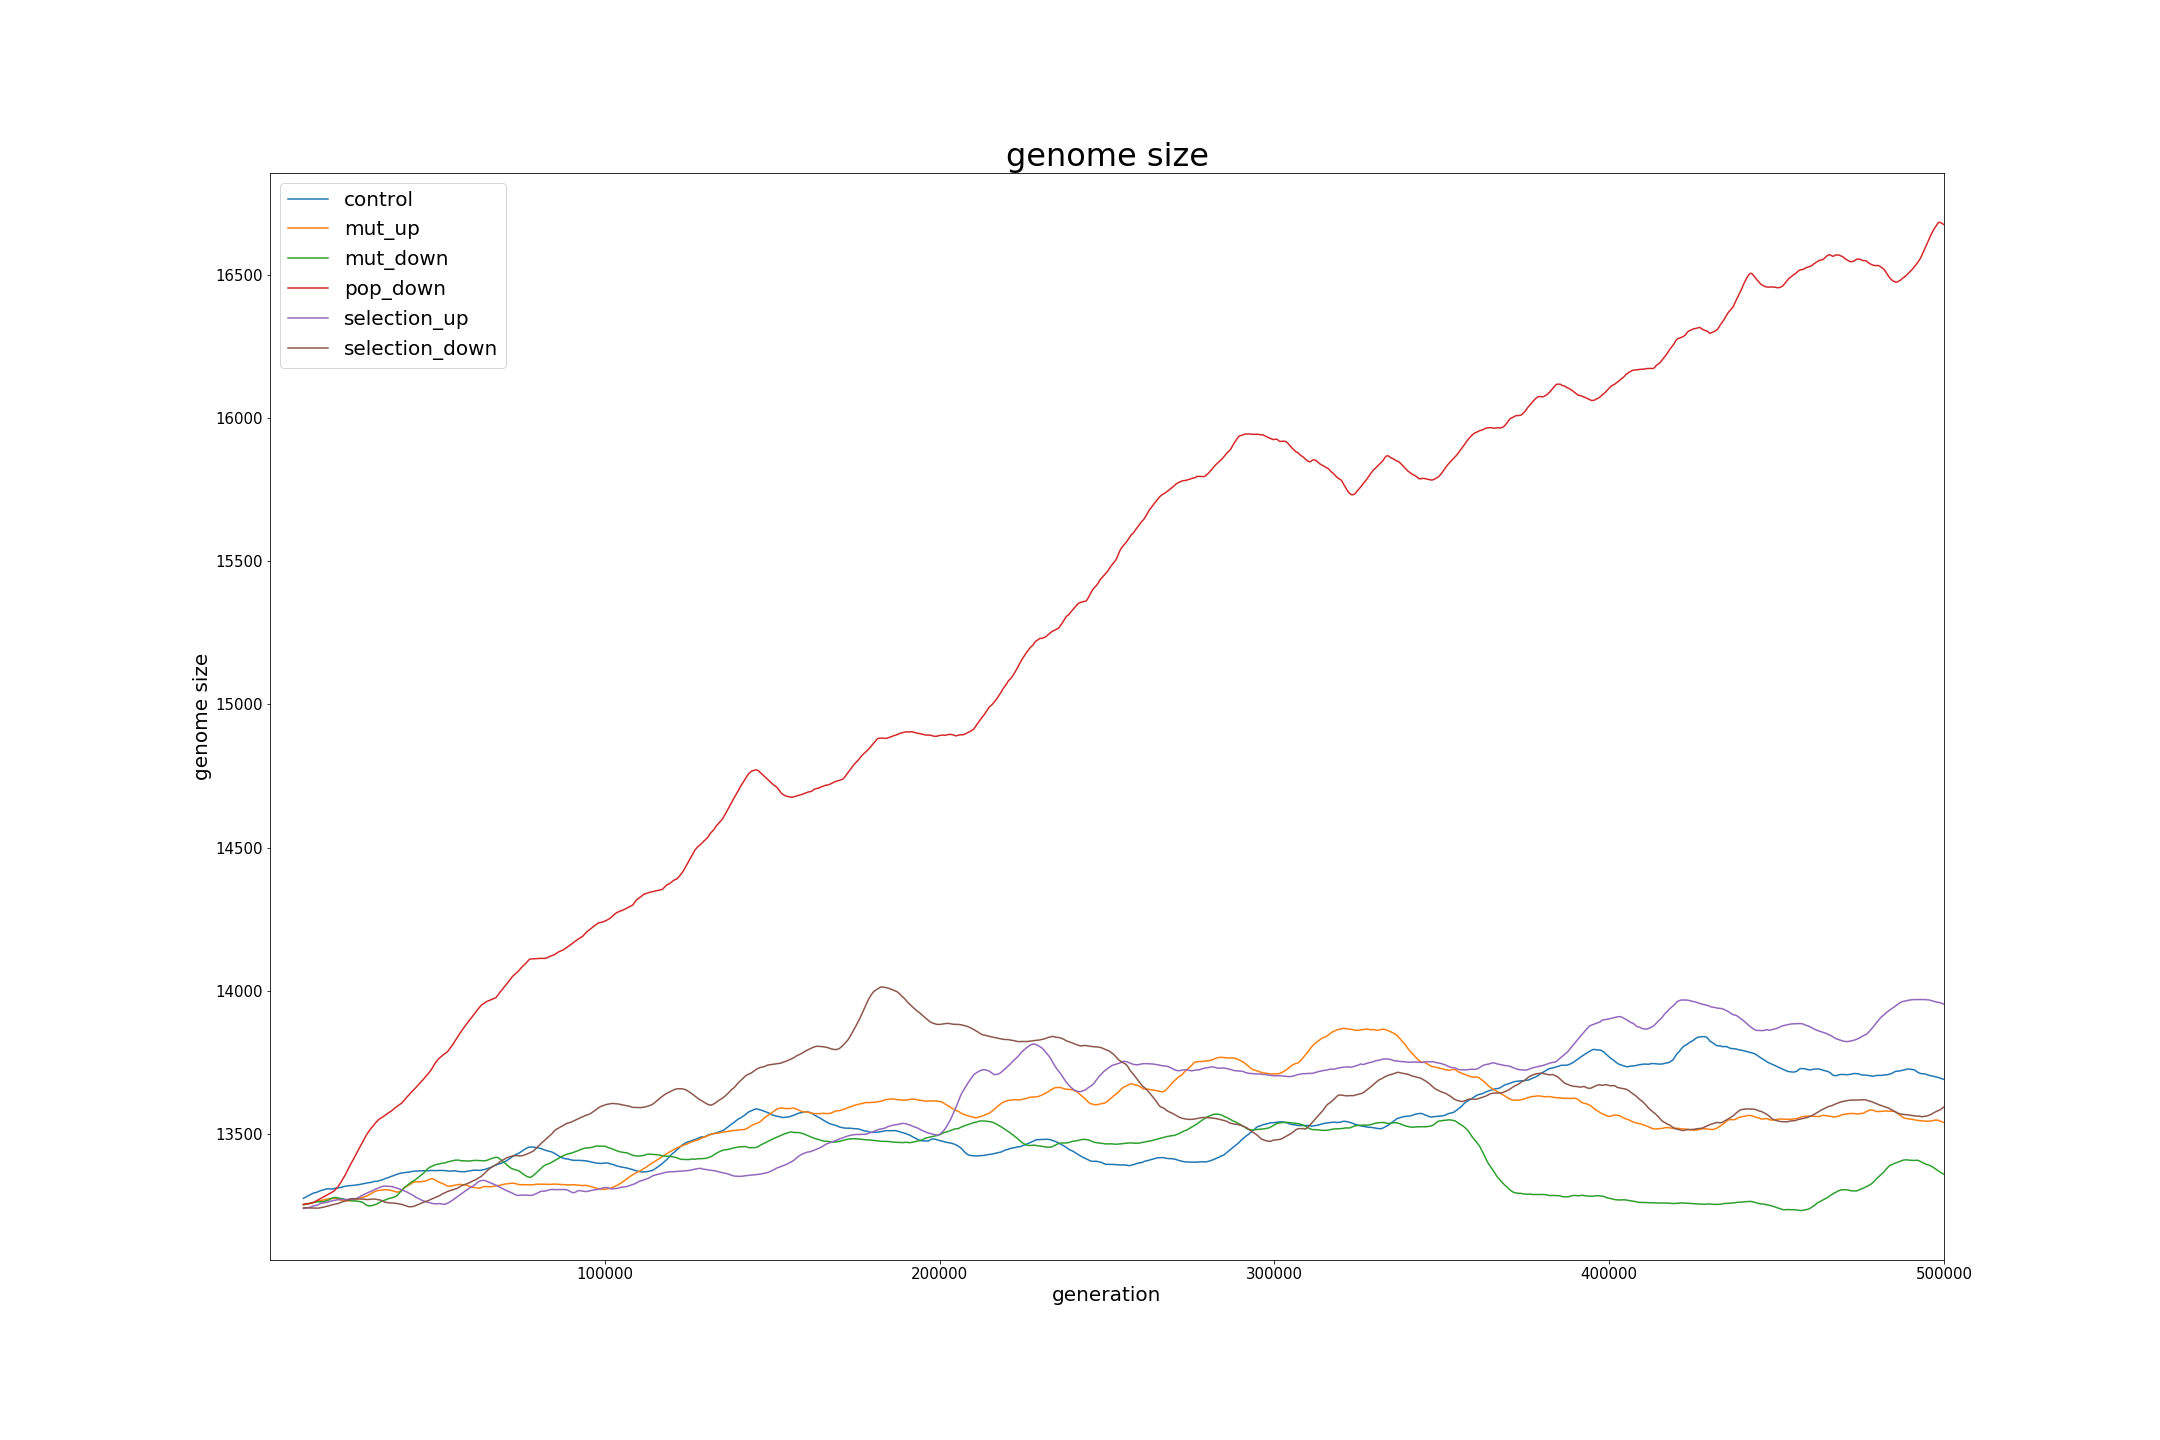
\includegraphics[width=\linewidth]{stat_fitness_global_mean_genome_size}
	\centering
	\caption[Genome size]{Genome size in number of bases of all conditions. Average taken across all five seeds for each condition.}
	\label{fig:genome_size}
\end{figure}
In fact the \textit{population down} condition had a runaway increase in the number of bases, reaching over 16,500 bases, at least a 25\% increase over the original wild type's roughly 13,200. Surprisingly, even after 500,000 generations it seems that the upper limit may still not have been reached. 

The next obvious observation is that of the remaining conditions, only the \textit{selection up} condition seems to have made much of a significant change with its 11\% increase. All of the remaining conditions had a mild increase in genome size. 

Also noteworthy is that the mutation down condition appears to have had a steady increase in the number of base pairs until a maximum of just over 14,000 around generation 350,000 before having a fairly sharp decline back to nearly the original size. 

\subsection{Metabolic Error and Fitness}
Figures ~\ref{fig:mean_fitness_plot} shows the mean fitness of the population for the control, mutation up/down, and population down conditions. Selection up/down were excluded from this graph because they were significantly outside of the range of the other conditions, but they are included in Figure~\ref{fig:mean_fitness_barchart}, a histogram of the results.

\begin{figure}[H]
	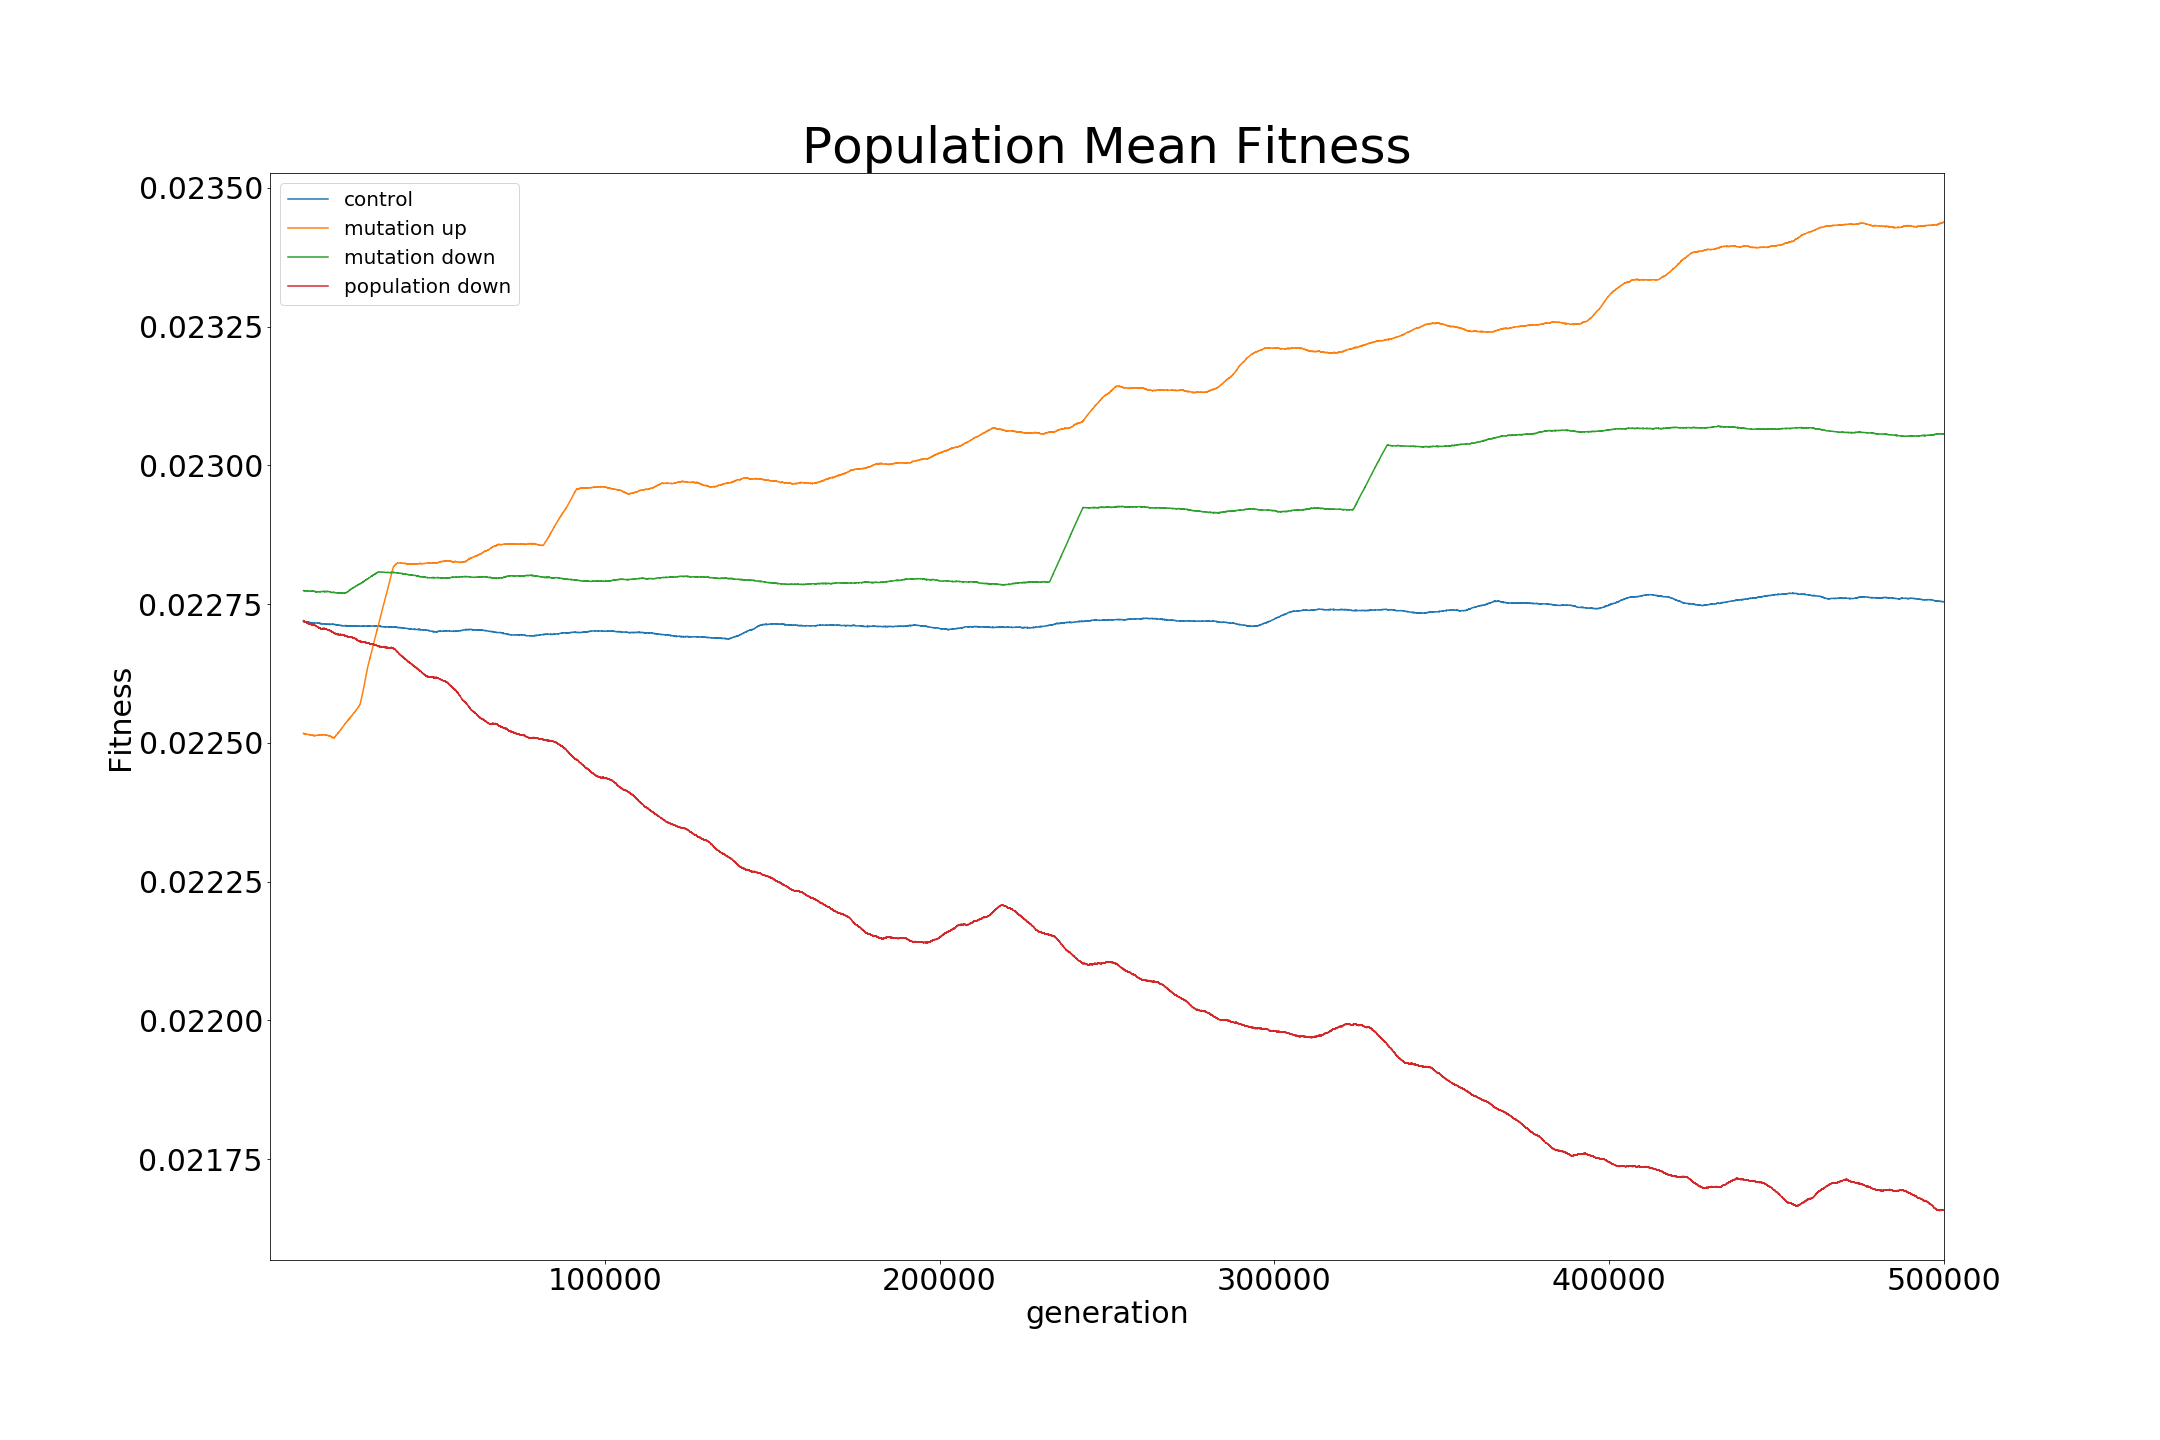
\includegraphics[width=\linewidth]{population_mean_fitness_chart}
	\caption[Mean fitness]{Plot of the mean fitness over time for the control, mutation up/down, and population down conditions.}
	\label{fig:mean_fitness_plot}
\end{figure}

We can see in the figure that the fitness of the control condition (in blue) pretty consistently stayed at the same level, likely owing to the fact that the wild genotype had already been allowed to evolve for 10 million generations in this environment, so the phenotype closely lines up with the target before the simulations even began. Small fluctuations occurred due to mutations, insertions, etc. but the average fitness remained steady. 

More interesting is the population down condition, where the average fitness in the whole population pretty sharply declined. 

\begin{figure}[H]
	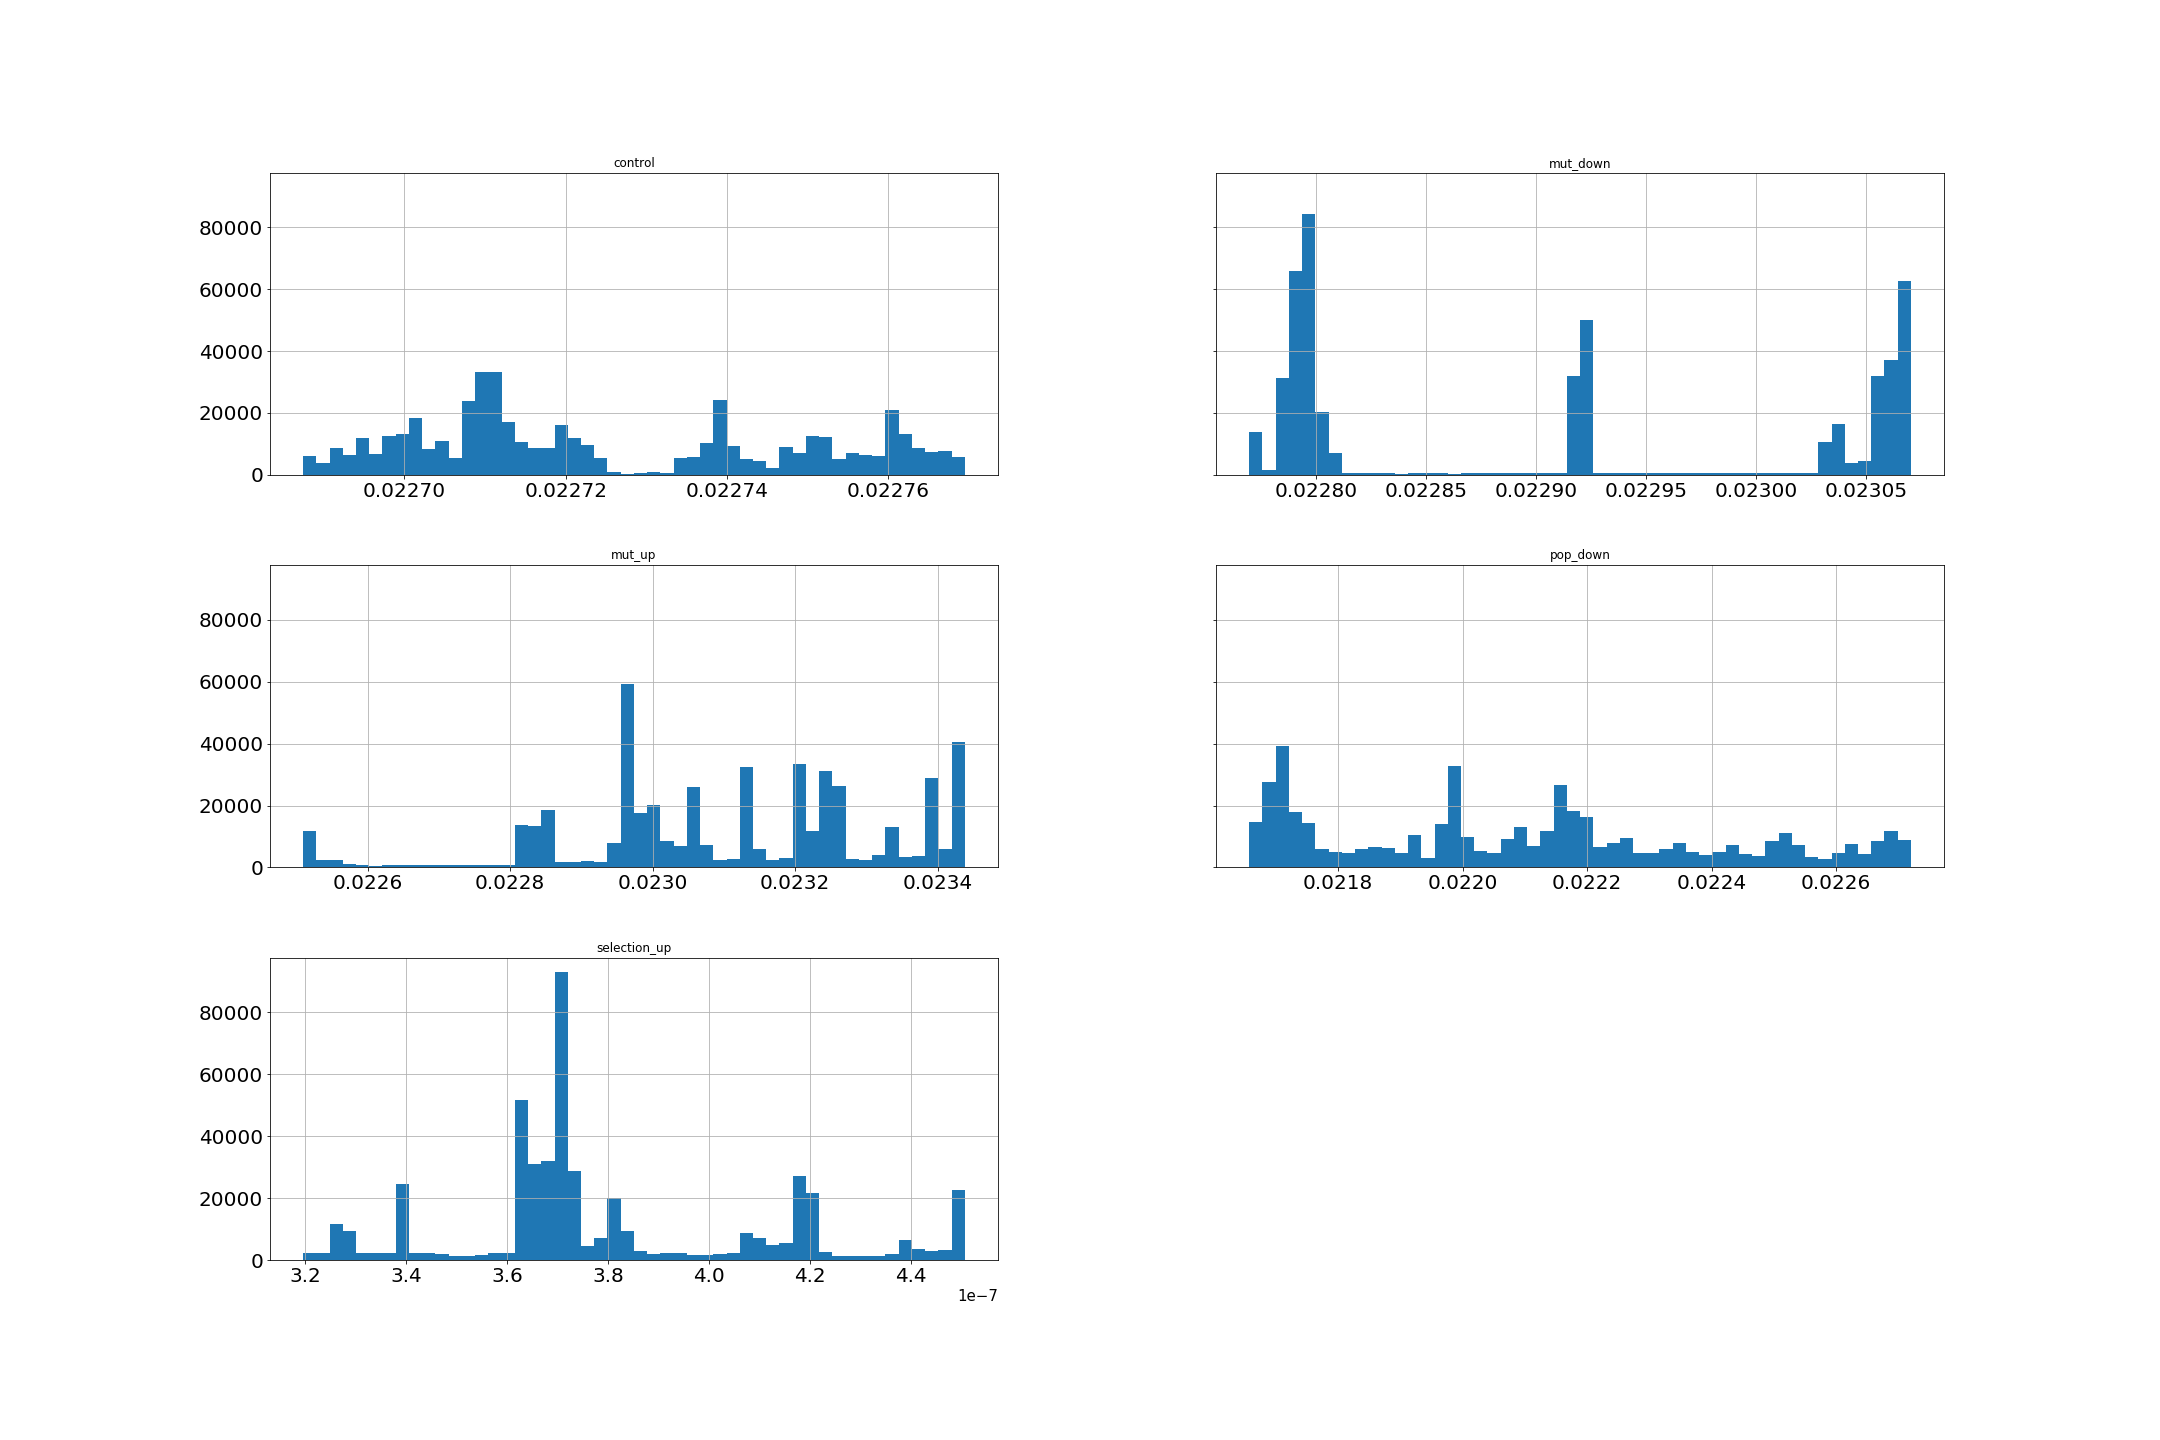
\includegraphics[width=\linewidth]{fitness_barchart}
	\caption[Mean fitness bar chart]{Bar chart of all conditions' fitness.}
	\label{fig:mean_fitness_barchart}
\end{figure}
Figure~\ref{fig:mean_metabolic_error} shows the mean metabolic error across all seeds for the whole population over time with respect to each condition. 
\begin{figure}[H]
	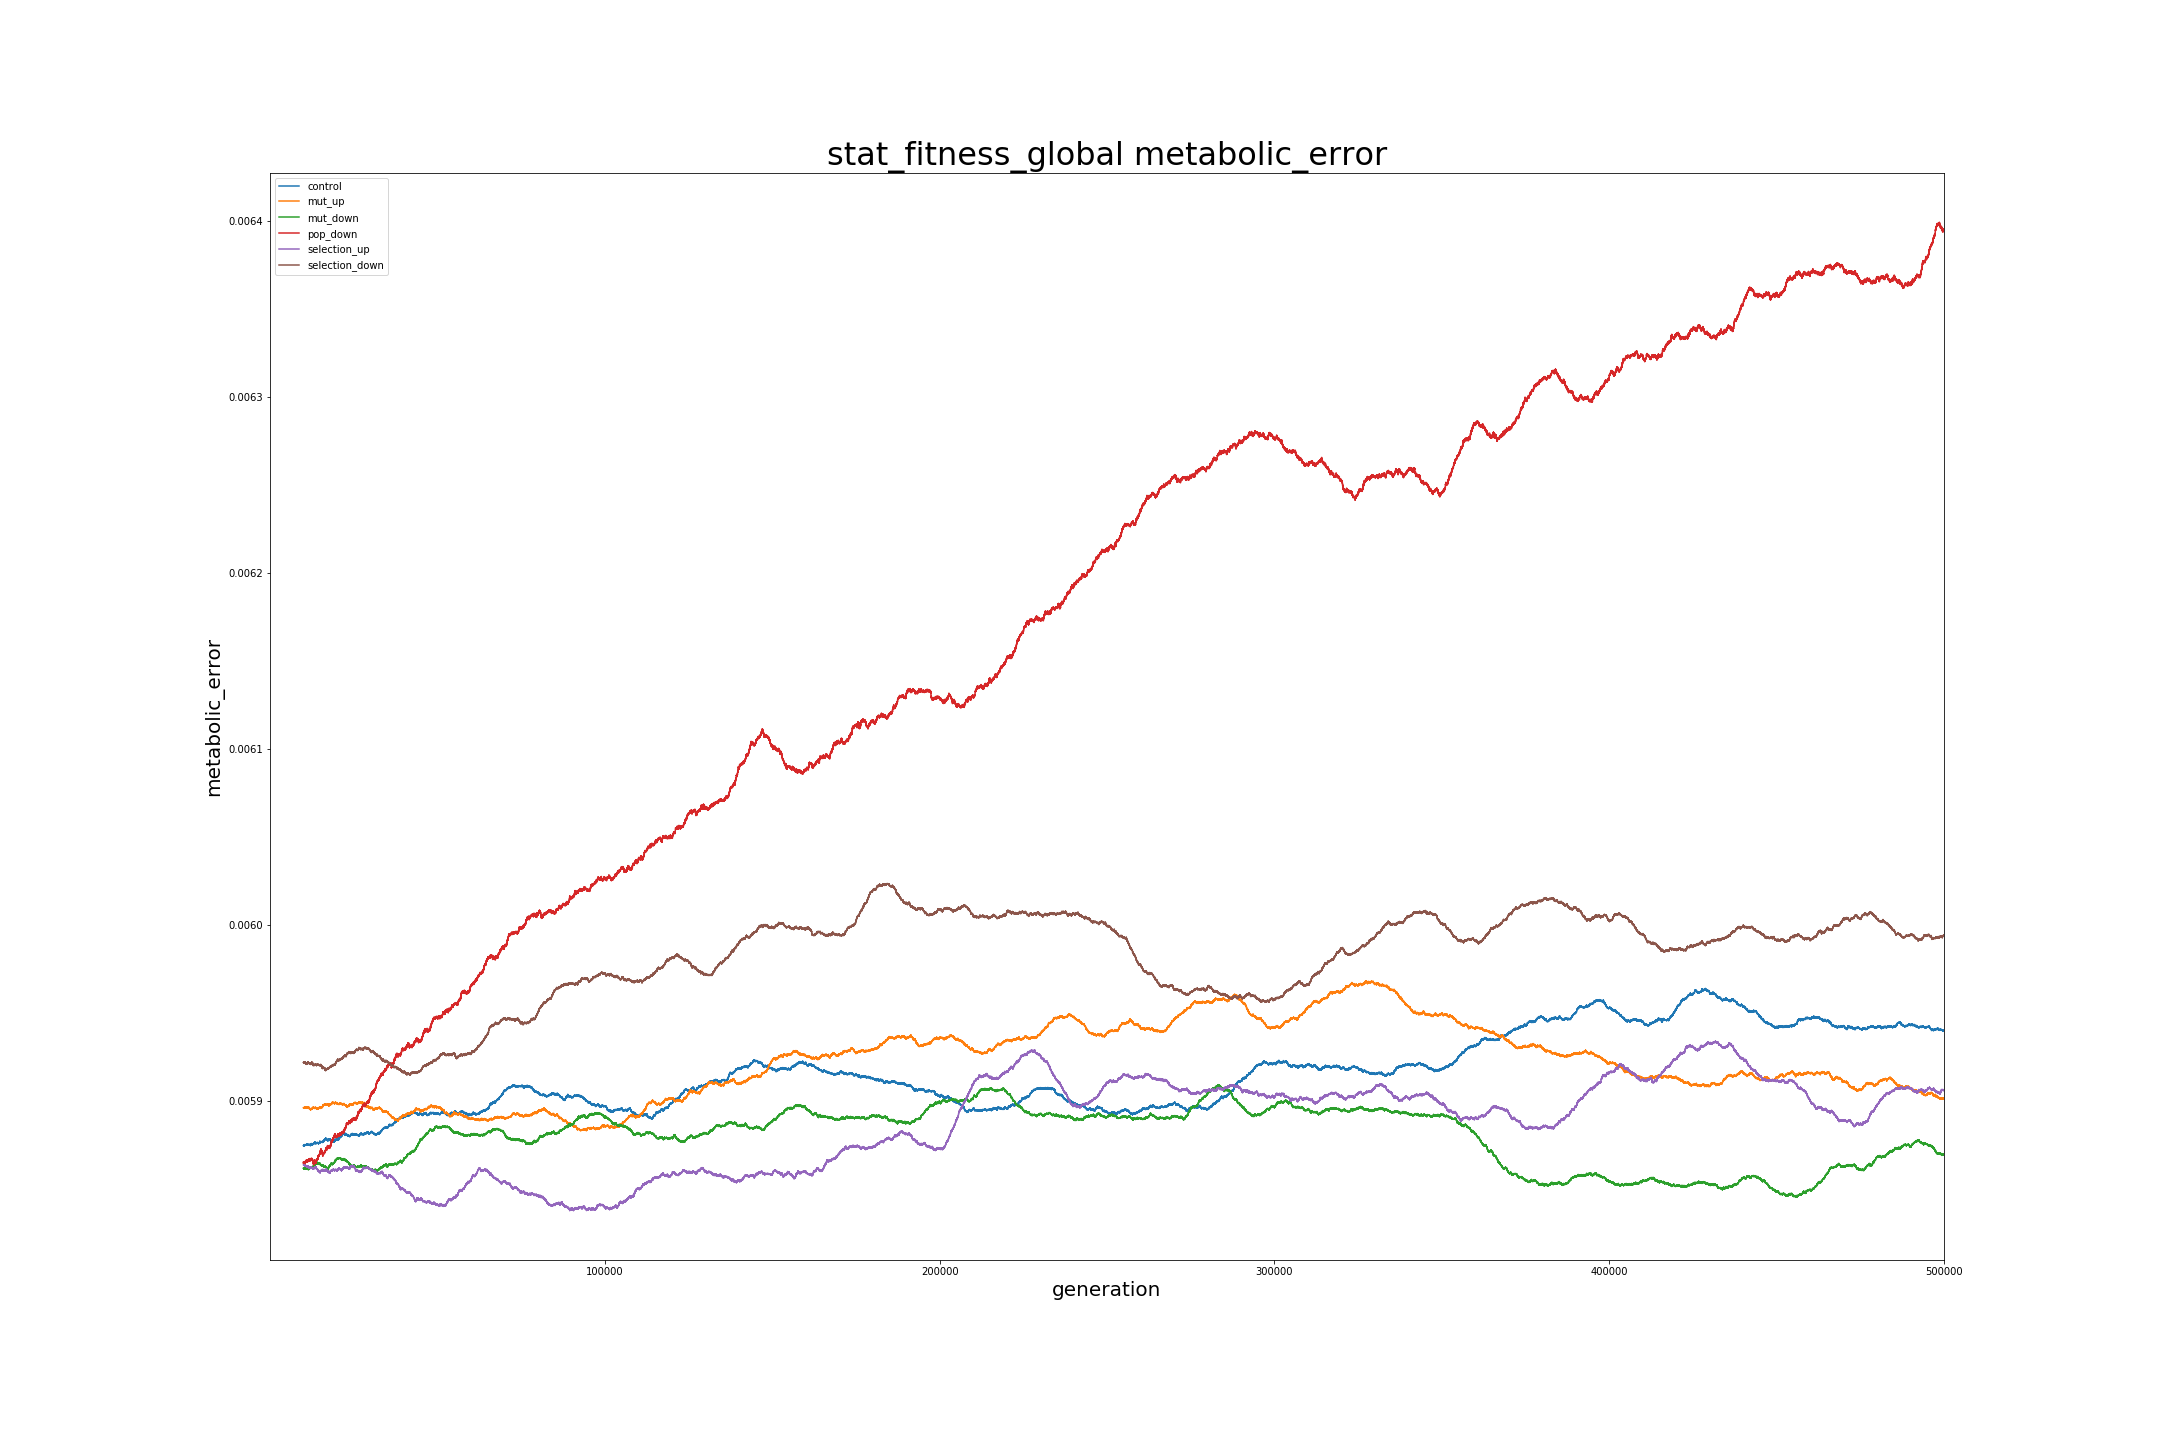
\includegraphics[width=\linewidth]{stat_fitness_global_mean_metabolic_error}
	\caption[Metabolic error]{Plot of the metabolic error over time for all conditions, average of all seeds}
	\label{fig:mean_metabolic_error}
\end{figure}



It seems that with the smaller population size, genetic drift may be more strongly at work in continually increasing the gap between the phenotype and environmental function, as the lack of variety inherent in a smaller population causes a cascade of increasingly deleterious consequences. 

Table~\ref{table:fitness_means_std_dev} below gives the mean fitness scores for differing conditions. The selection up/down conditions seem to be somewhat anomalous.
\begin{table}[H]
	\centering
	\begin{tabular}{|c||c|c|}
		\hline
		& \textbf{mean} & \textbf{standard deviation} \\
		\hline \hline
		control & 0.022725416617759595 & 2.3443283583311204e-05 \\
		\hline
		mutation up & 0.02310700617283088 & 0.00021918255246890017 \\
		\hline
		mutation down & 0.022908786914463554 & 0.0001180940074554785 \\
		\hline
		selection up & 3.803823317637301e-07 & 3.130503751740127e-08 \\
		\hline
		selection down & 0.3695935240107418	& 0.0008101731945386823 \\
		\hline
		population down & 0.02209722426327717 & 0.00031042637566743275 \\
		\hline
	\end{tabular}
	\caption[Fitness means and standard deviations.]{Fitness means and standard deviations. }
	\label{table:fitness_means_std_dev}
\end{table}

\subsection{Genome Structure}
In this section we examine the effects of the differing conditions on the structure of the genome as measured by the criteria in Tables~\ref{table:aevol_stats_genes_and_bp} and~\ref{table:aevol_stats_fitness_and_mutation}. 

\subsubsection{Non-coding DNA}
One important factor in genome structure is the amount of non-coding DNA, i.e. the number of bases which are part of a genome but which do not encode protein sequences. In the case of aevol, this means 
\begin{figure}[H]
	\centering
	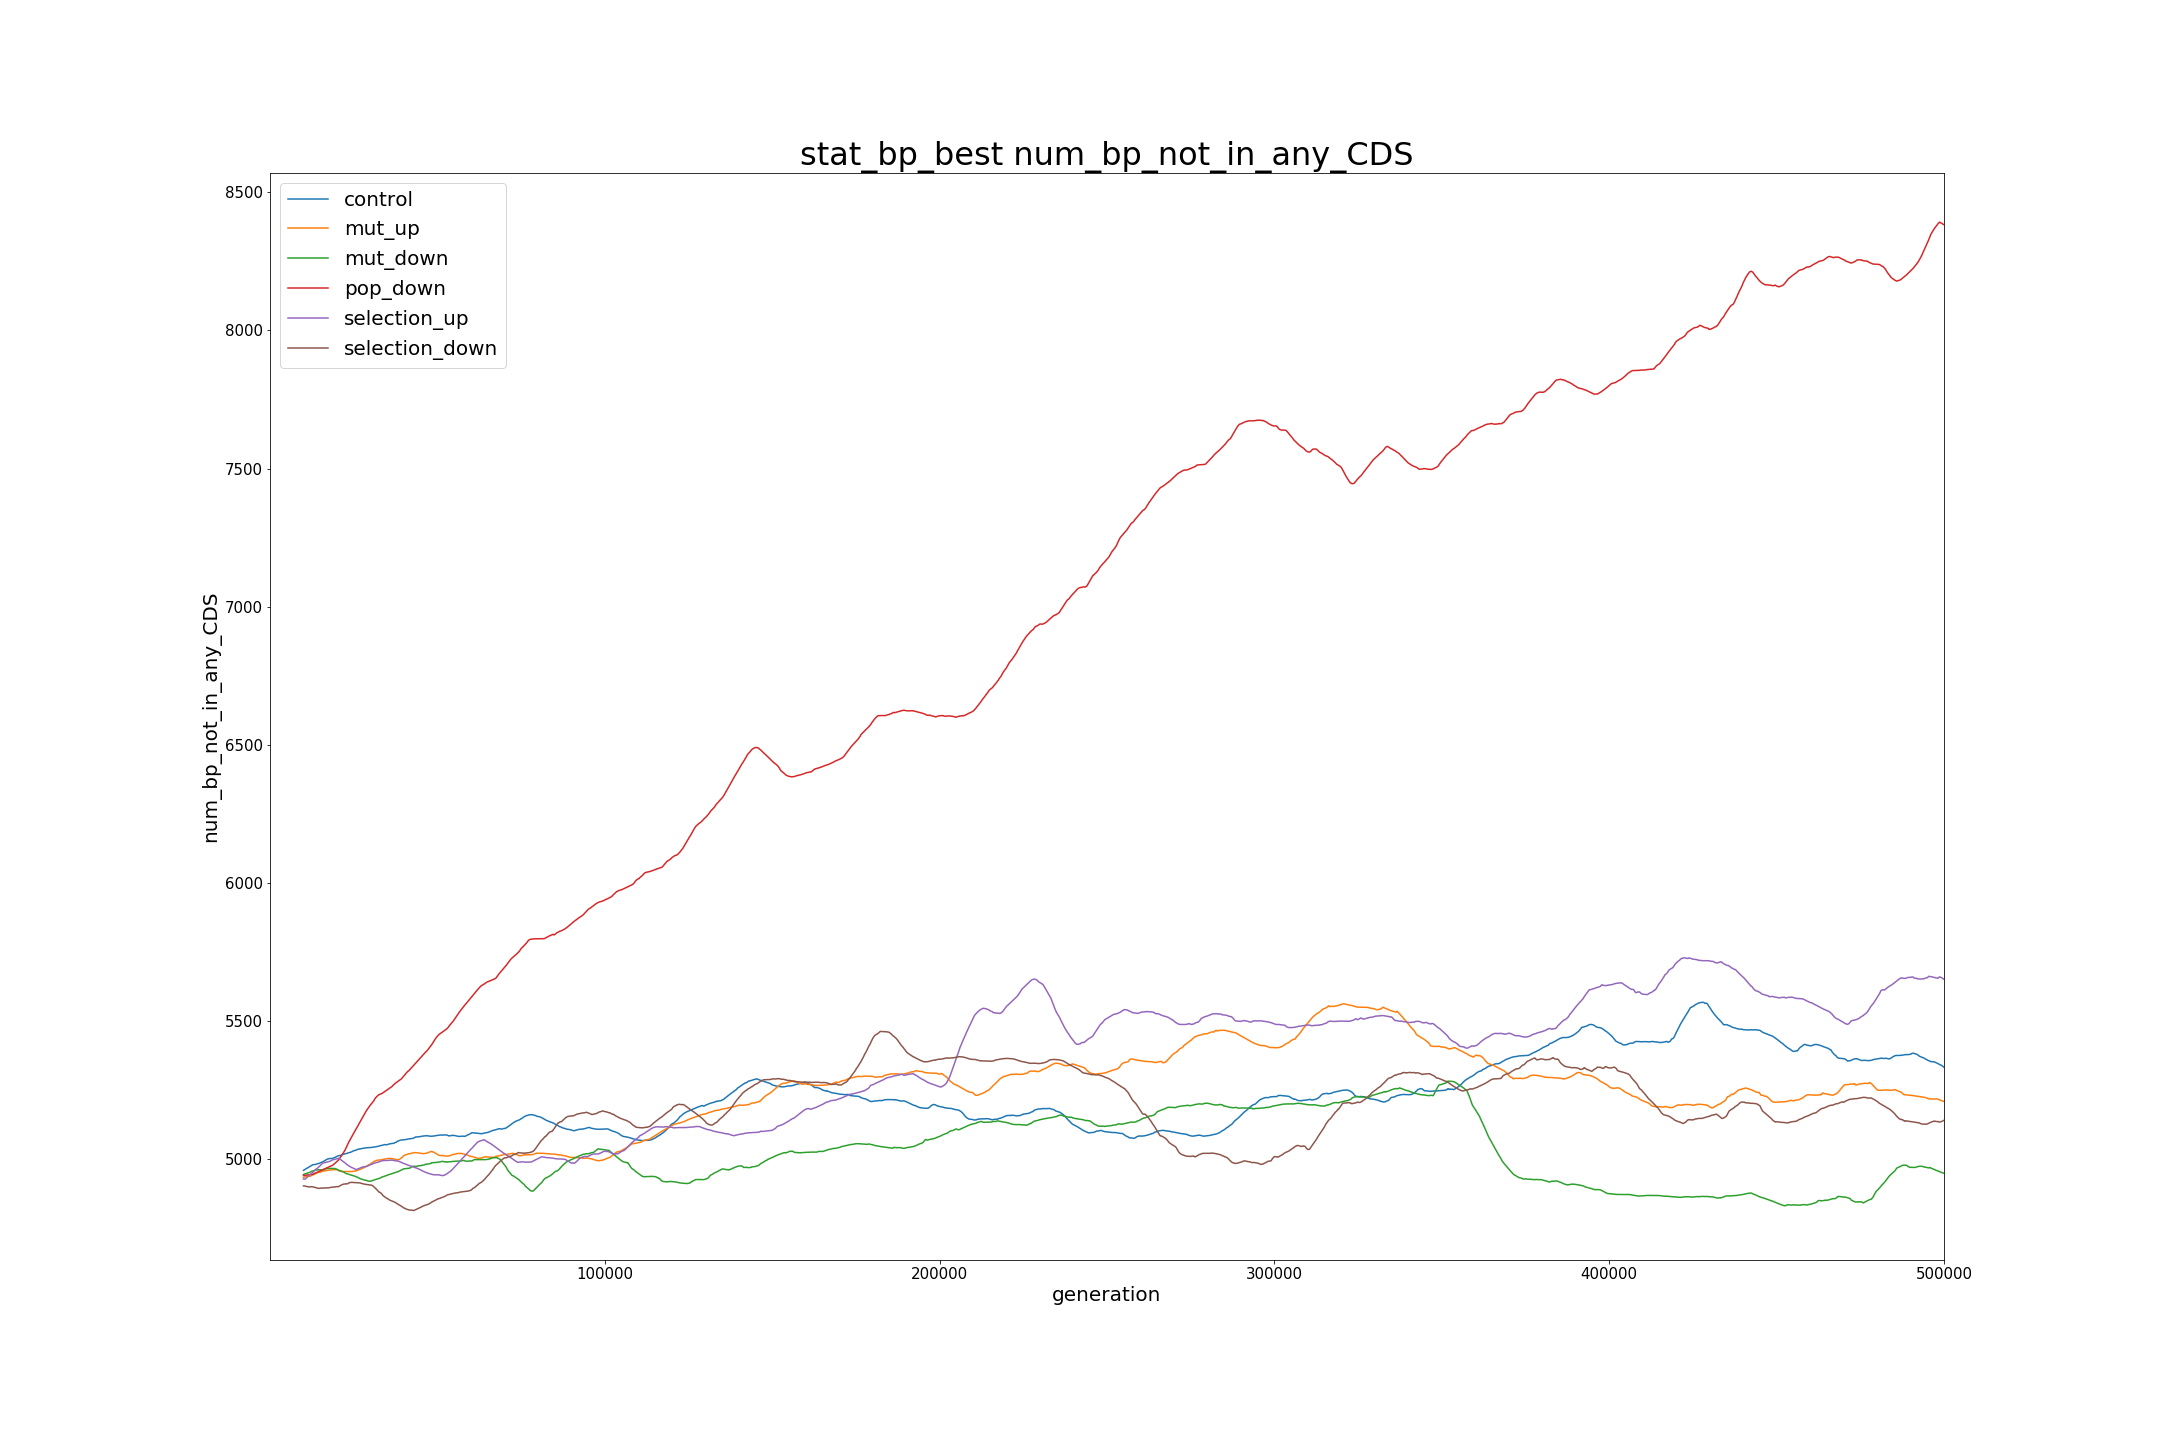
\includegraphics[width=\linewidth]{stat_bp_best-mean_num_bp_not_in_any_CDS}
	\caption[Non-coding DNA]{Plot of non-coding DNA over time for all conditions, average of all seeds.}
	\label{fig:mean_non-coding_DNA}
\end{figure}

\subsubsection{Number of Genes}\label{sec:number_of_functional_genes}
Figure~\ref{fig:mean_num_functional_genes} below illustrates the mean number of genes across the population for each condition.  
\begin{figure}[H]
	\centering
	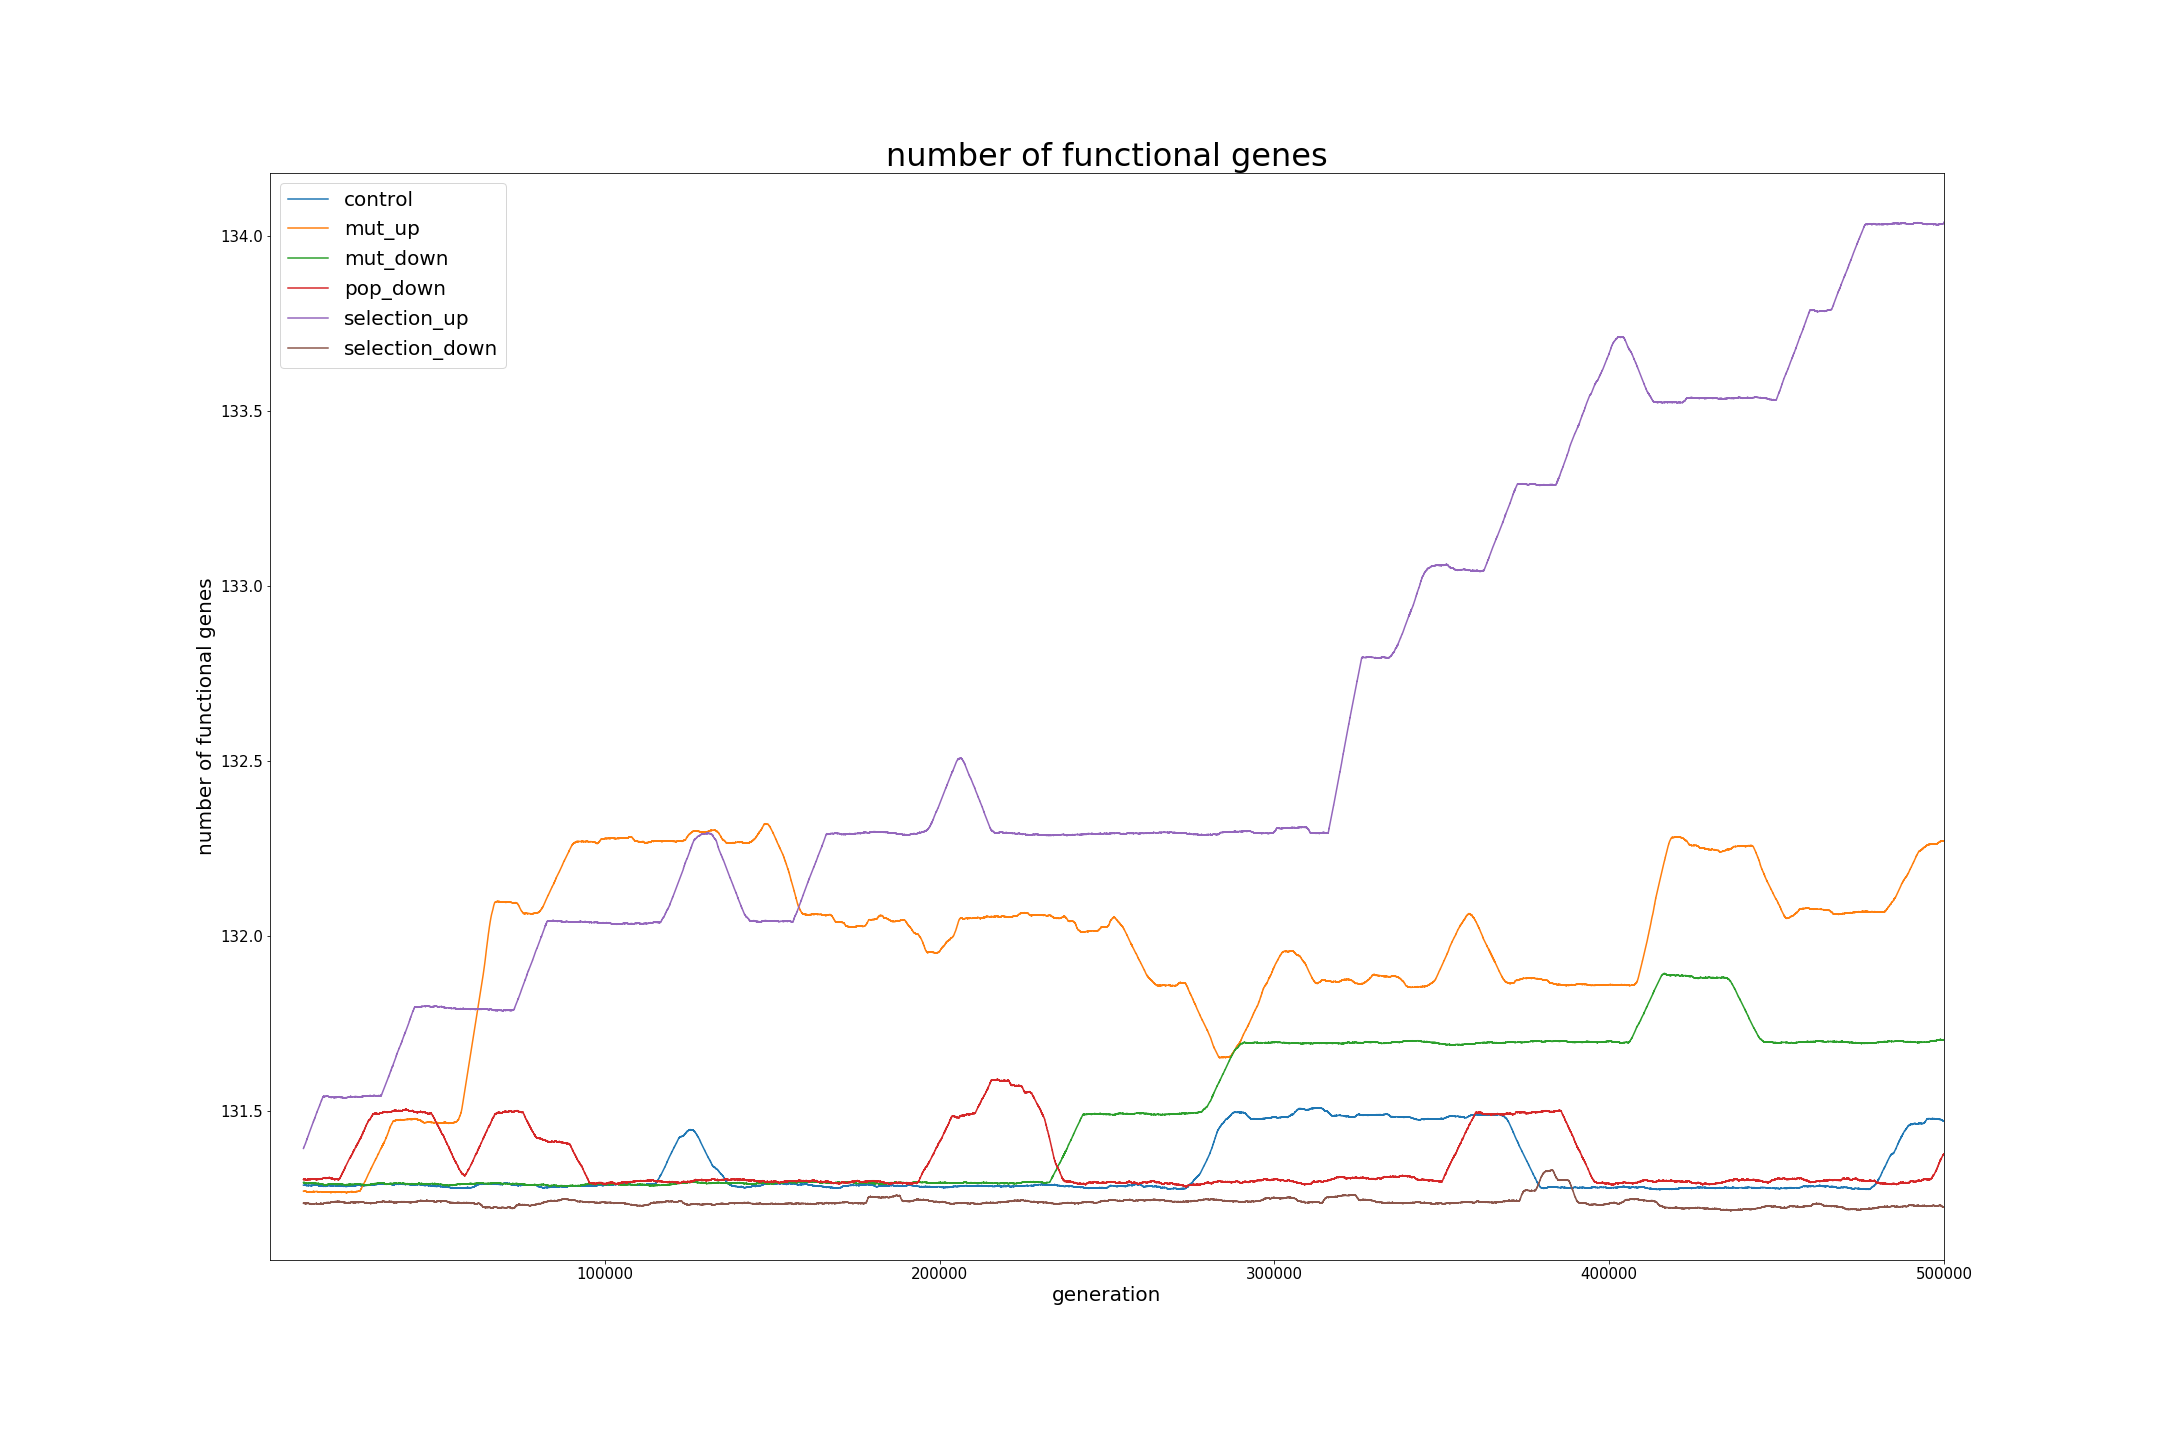
\includegraphics[width=\linewidth]{stat_genes_global_mean_num_functional_genes}
	\caption[Mean number of functional genes]{Plot showing the mean number of functional genes over time across all seeds.}
	\label{fig:mean_num_functional_genes}
\end{figure}
As seen in the figure, the increased selection condition showed the greatest increase in the number of functional genes in the whole population, about 3\% (130 to 134). Interestingly, the selection down condition did not change the number of genes at all, which is to be expected, since with a lower selection pressure, any newer genes may not be selected for reproduction. Whereas most of the other curves are fairly flat, the mutation up condition fluctuates relatively rapidly, owing to the quick increase and decrease in the number of base pairs. 

\subsubsection{Average Size of Functional Genes}\label{sec:average_size_functional_genes}
Figure~\ref{fig:mean_functional_gene_size} shows the average number of base pairs for each functional gene for the best individual, mapped out over the 500,000 generations. 
\begin{figure}[H]
	\centering
	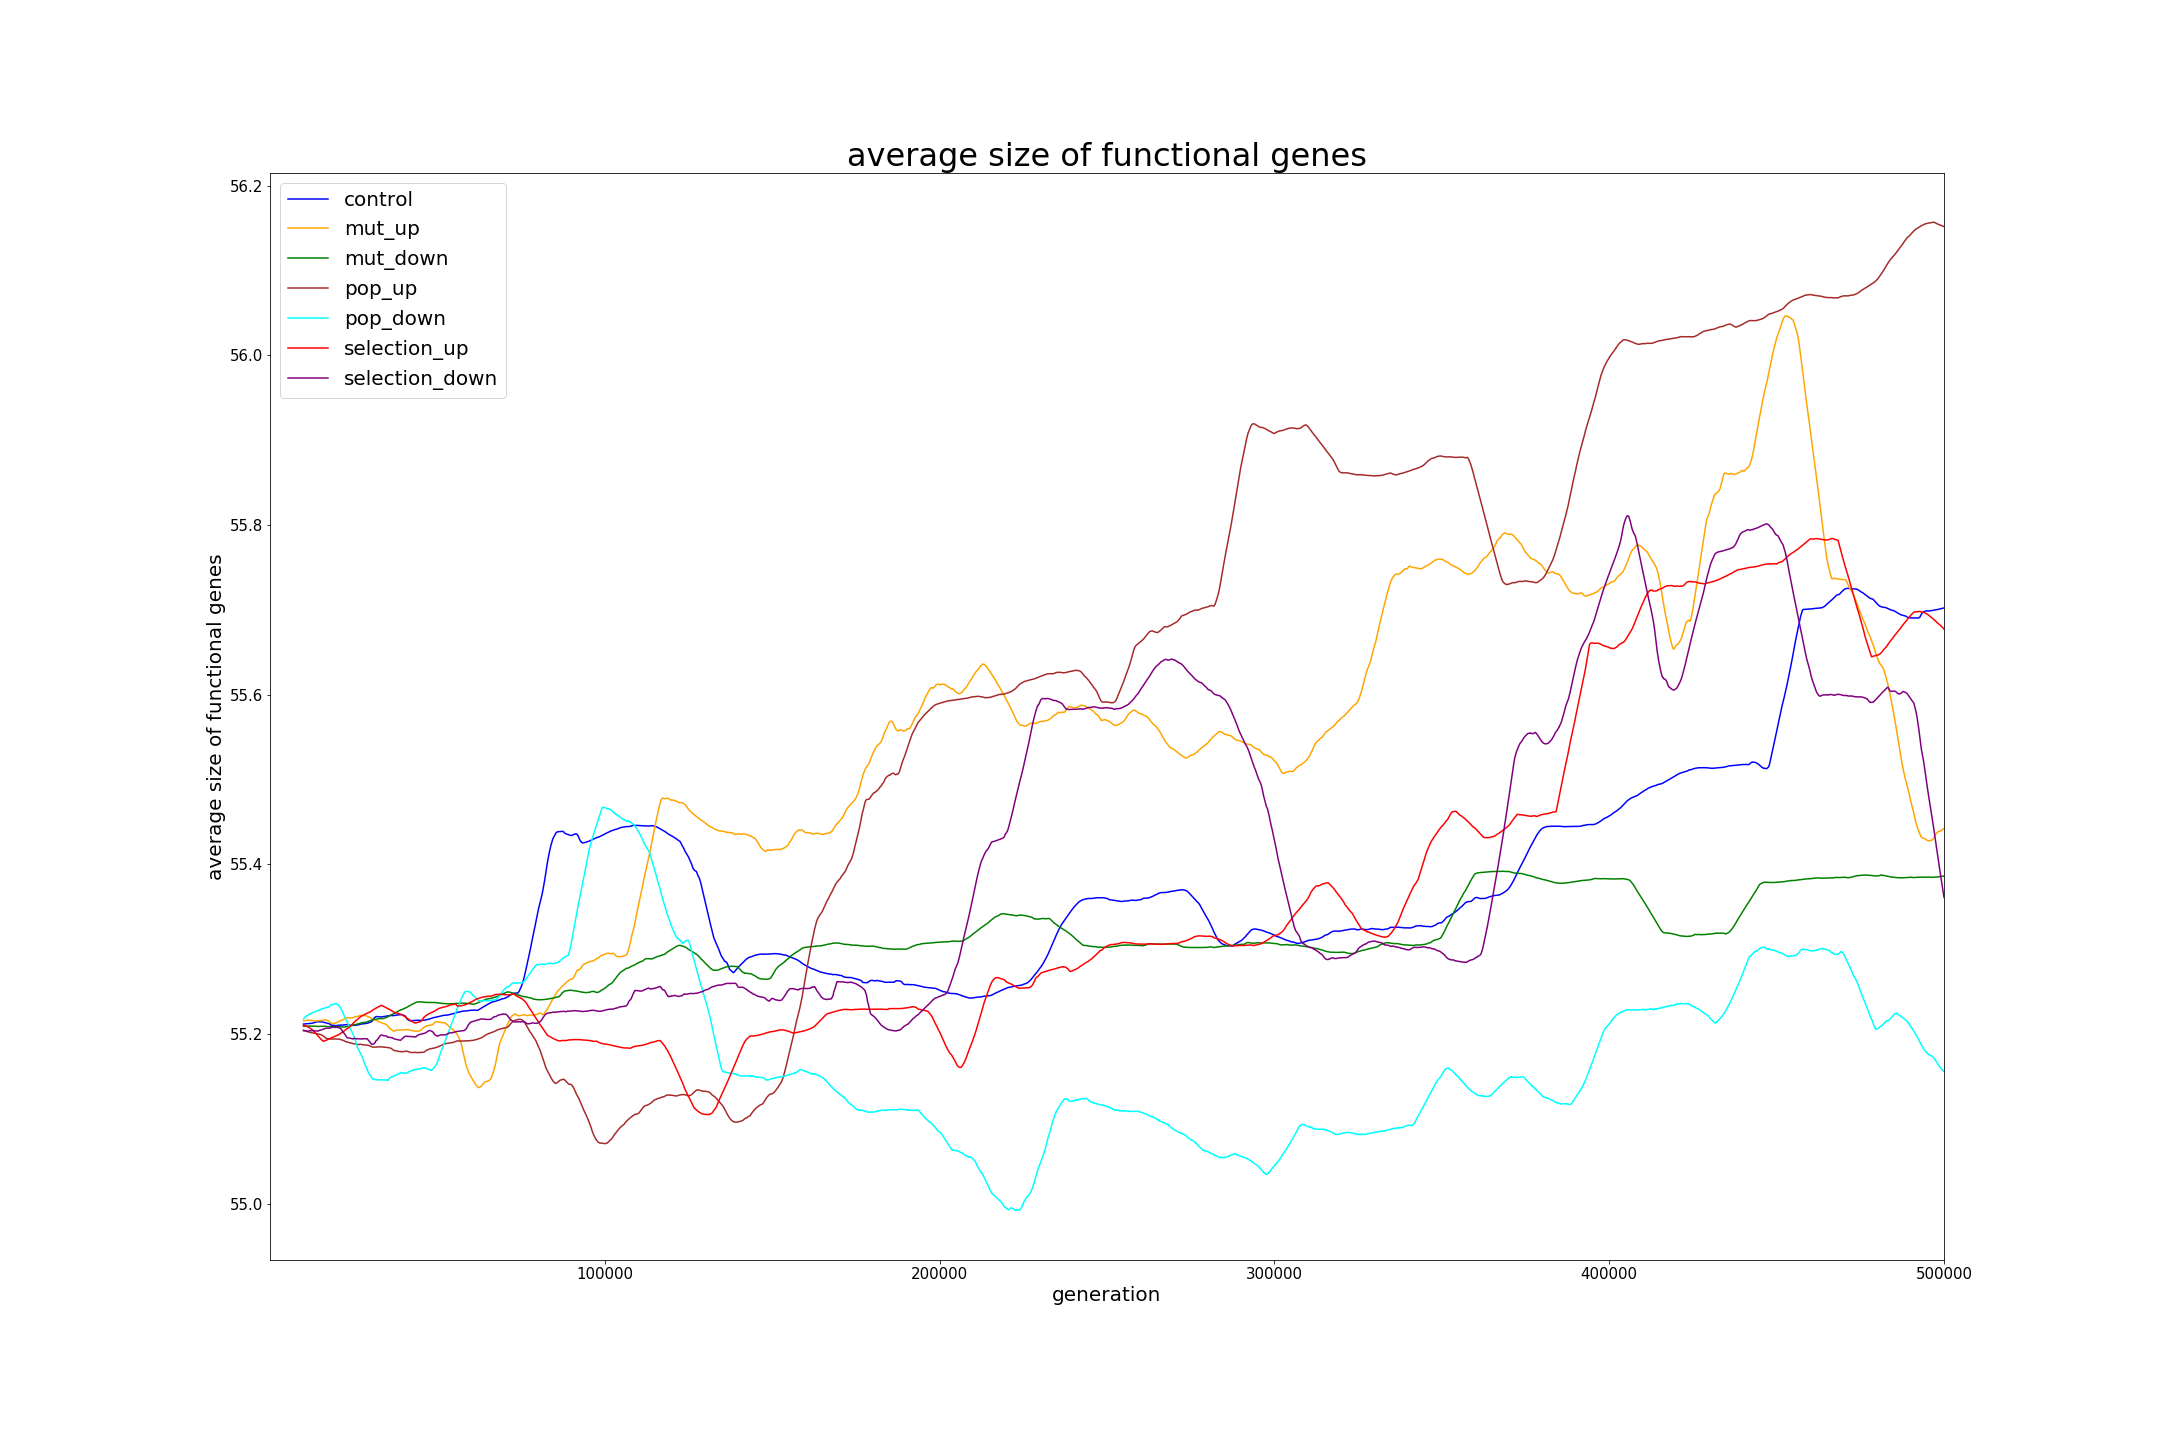
\includegraphics[width=\linewidth]{stat_genes_global_mean_avg_size_of_functional_genes}
	\caption[Average size of functional genes]{Plot showing the average size of functional genes over time for all seeds.}
	\label{fig:mean_functional_gene_size}
\end{figure}
The population down condition continues to be the outlier in terms of genome structure, with the average size of the functional genes remaining noticeably lower than for any other condition. It is worth pointing out, however, that the difference between the smallest average and the largest average is only 1 base pair. 

\subsection{Evolvability}
In Figure~\ref{fig:evolvability_mean} below, we see the results of the experiments on evolvability for the best individual's (at generation 500,000) lineage. 
\begin{figure}[H]
	\centering
	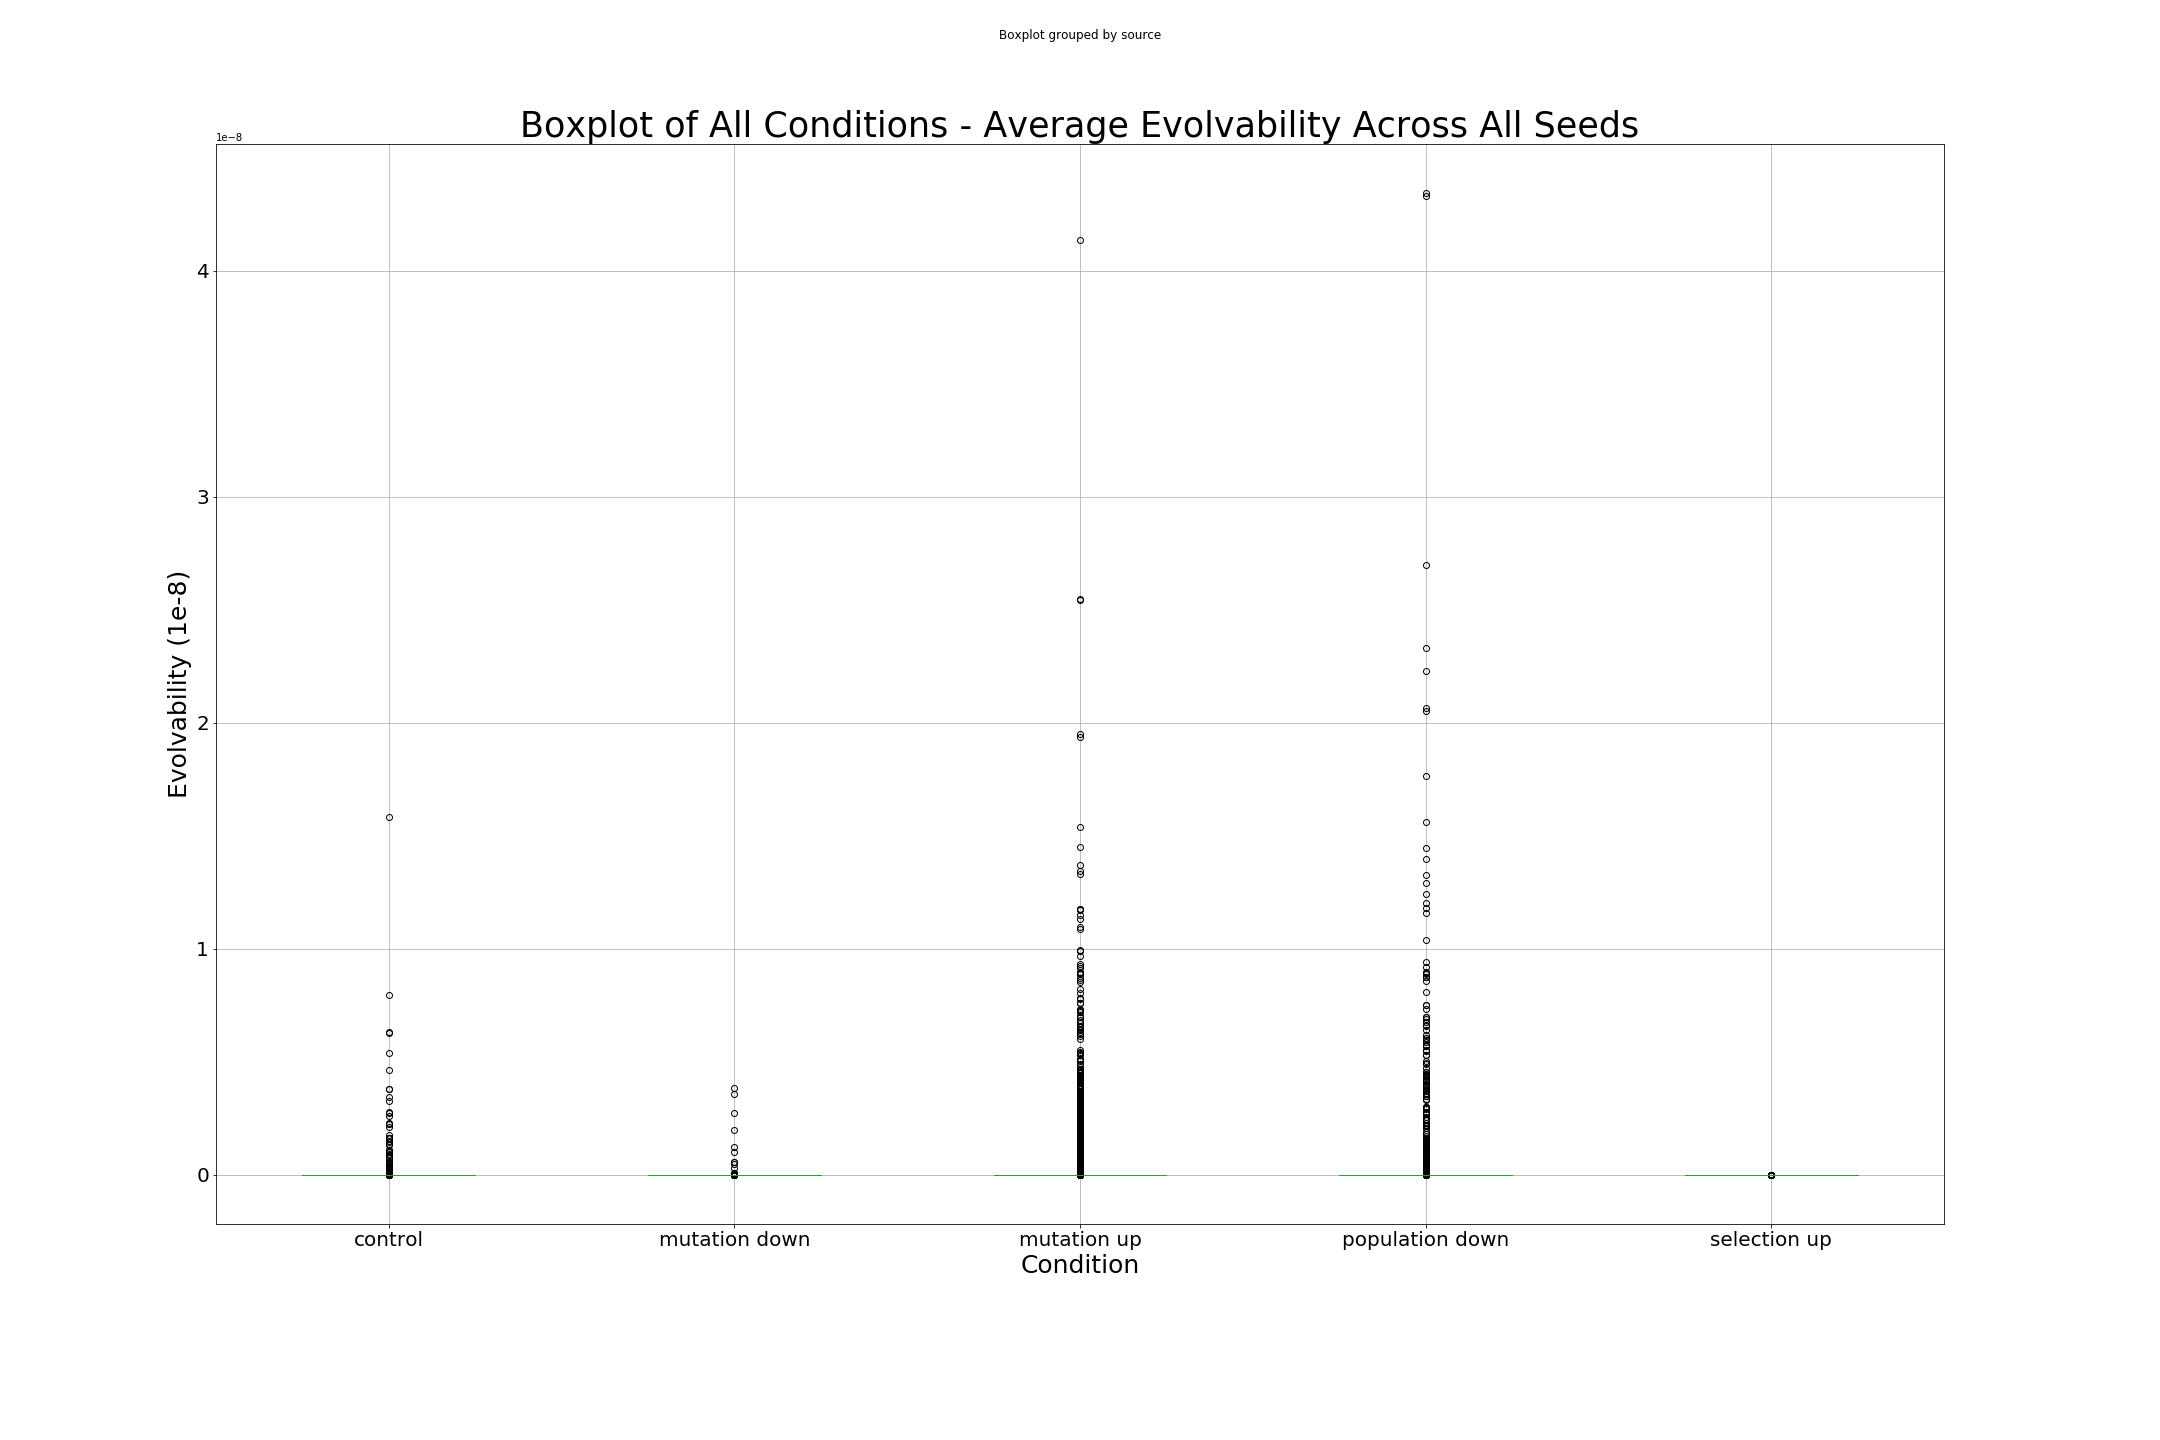
\includegraphics[width=\linewidth]{evolvability_boxplot_all_seeds_avg}
	\caption[Evolvability boxplot]{A box plot showing the mean evolvability spread of all seeds and all conditions. Higher numbers are more evolvable.}
	\label{fig:evolvability_mean}	
\end{figure}
The figure illustrates that, for each condition, overall the best individual still had quite low evolvability. For the selection up condition, however, the deviation from zero was even smaller, as illustrated in Table~\ref{table:mean_std_dev_evolvability} below, which provides the mean and standard deviation of the evolvability of the best individual in each condition. 

\begin{table}[H]
	\centering
	\begin{tabular}{| c | c | c |}
		\hline
		 & \textbf{mean} & \textbf{standard deviation}\\
		 \hline
		 \hline
		 control & 2.035523813975702e-11 & 3.2787490312081233e-10\\
		 \hline
		 $\mu_\text{up}$ & 9.97655150597127e-11 & 8.41749150634588e-10 \\
		 \hline
		 $\mu_\text{down}$ & 6.064697990806935e-12 & 1.2471674281540128e-10 \\
		 \hline
		 $k_\text{up}$ & 1.9498939718794653e-15 & 6.394659146405824e-14 \\
		 \hline
		 %TODO Fill in selection down
		 $k_\text{down}$ & & \\
		 \hline
		 $N_\text{up}$ & 8.837632116681012e-11 & 1.0799303682398726e-09 \\
		 \hline
		 $N_\text{down}$ & & \\
		 %TODO Fill in population down
		 \hline	 		 
	\end{tabular}
	\caption[Evolvability mean and standard deviation]{Table illustrating the mean and standard deviation of the evolvability for each condition. $\mu$ is the mutation rate, $k$ is the selection rate, and $N$ is the population size.}
	\label{table:mean_std_dev_evolvability}
\end{table}
\subsection{Robustness}
Recall from Section~\ref{subsec:robustness_antirobustness} that robustness is measured by the fraction of neutral mutants of an individual. In the following figure, we see a bar plot showing the spread of neutral mutants for the best individual for the control condition as well as the six variations. 

%TODO update graphic with more conditions once experiments are completed
\begin{figure}[H]
	\centering
	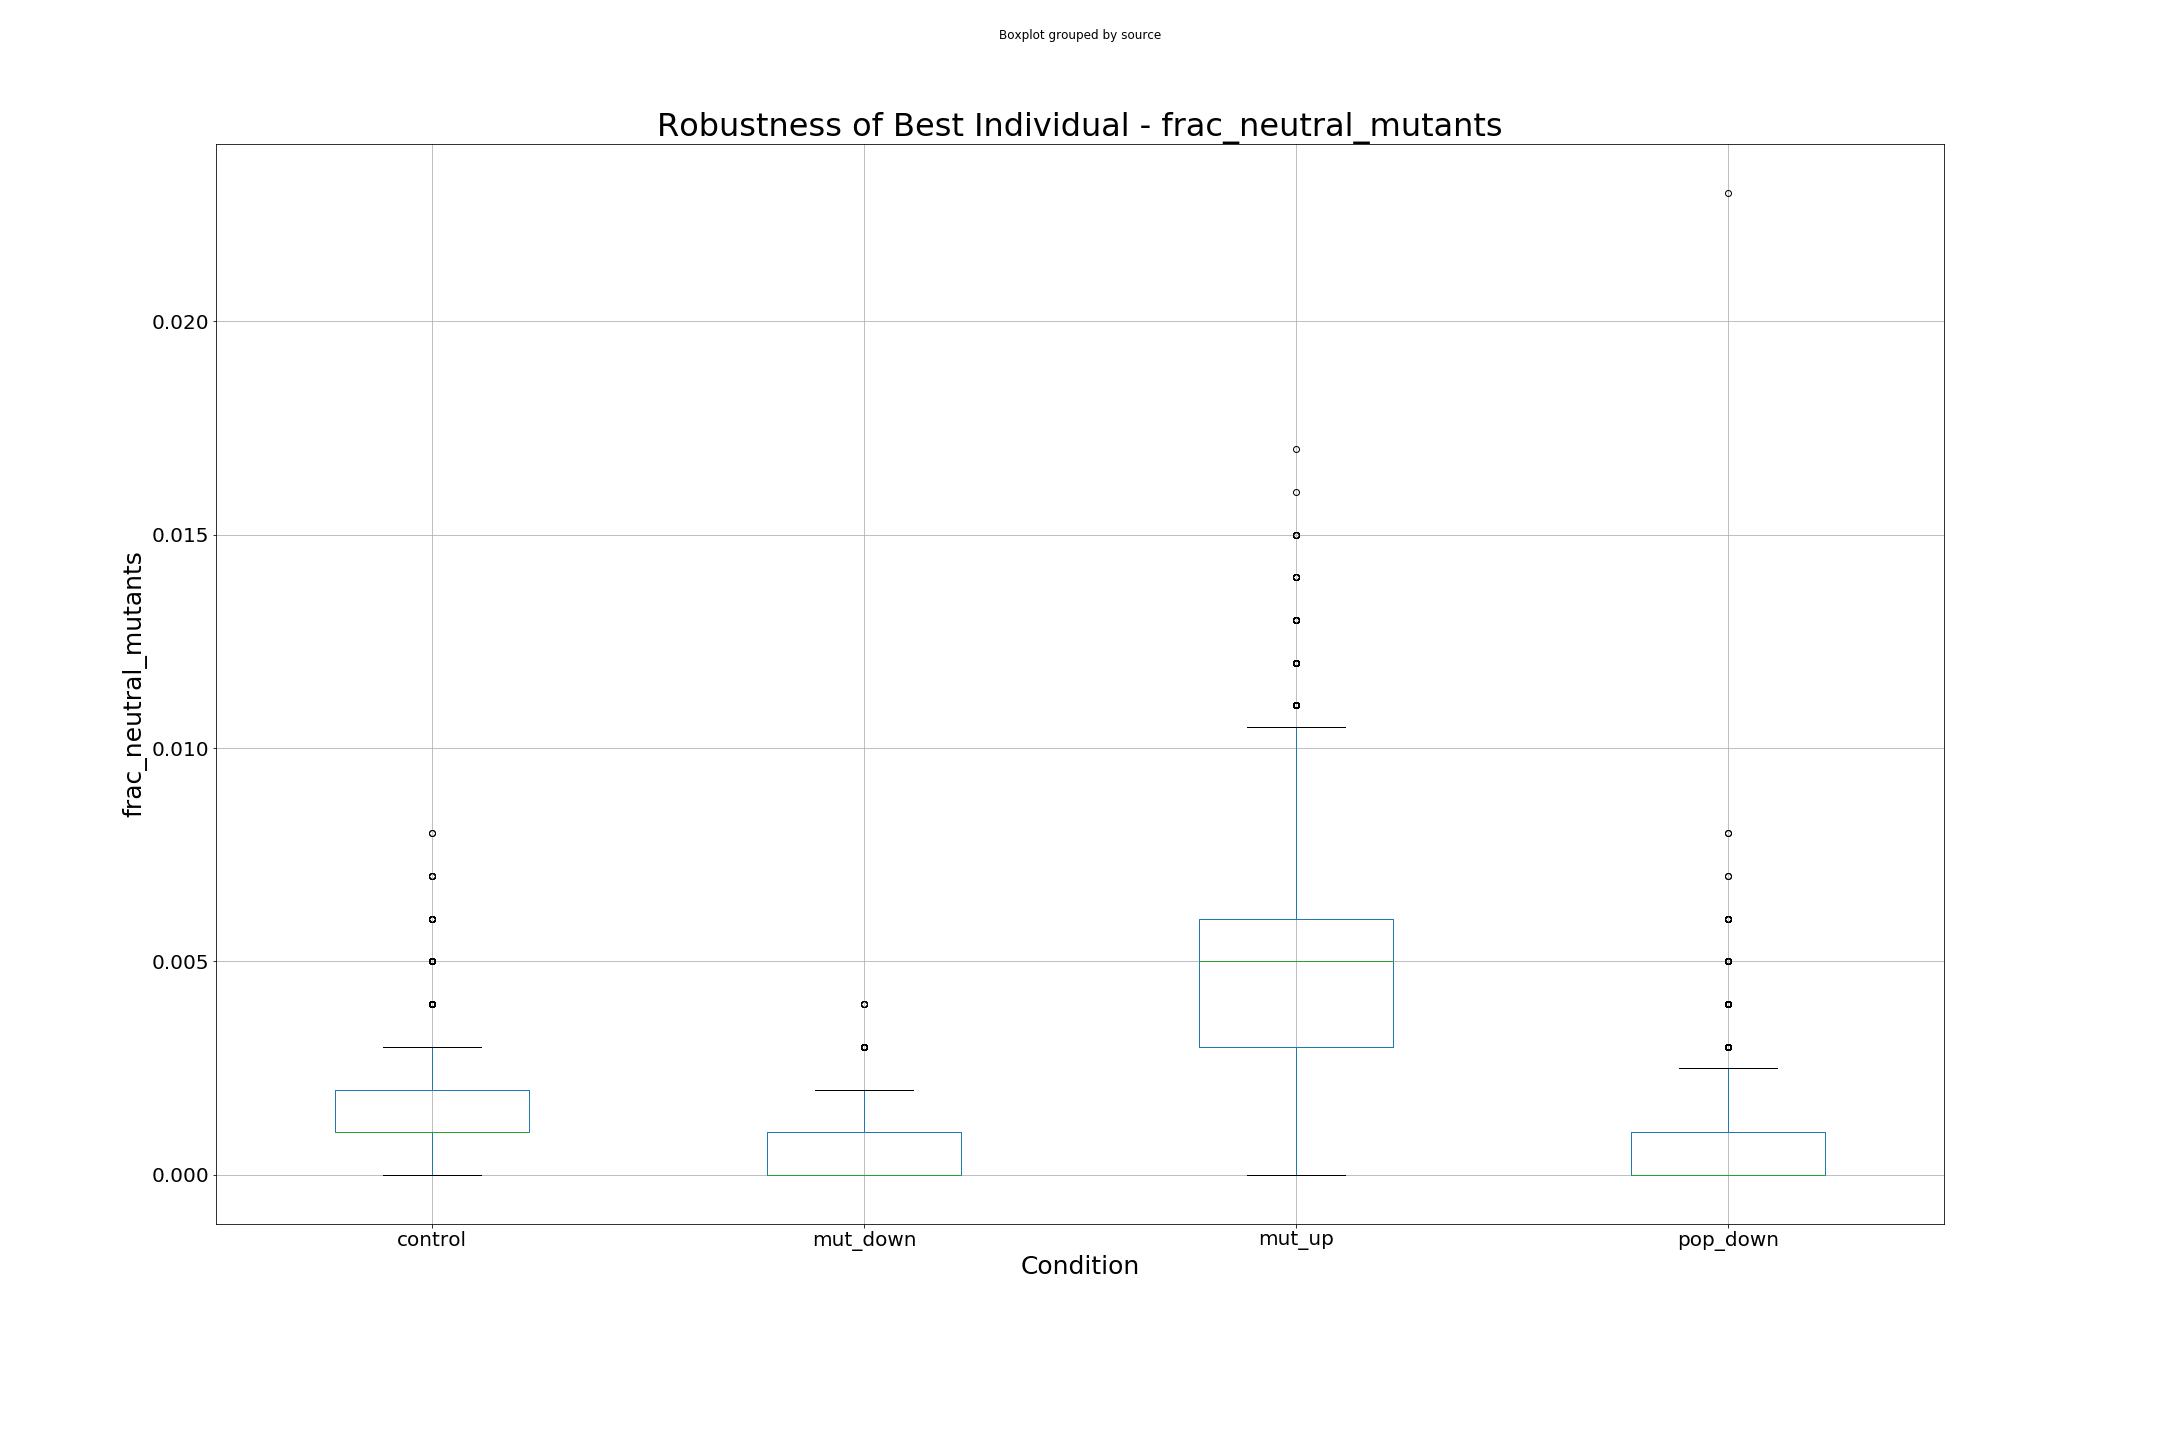
\includegraphics[width=\linewidth]{stat_robustness_best_mean_frac_neutral_mutants}
	\caption[Robustness bar graph]{Bar graph showing the spread of neutral mutants for the best individual at generation 500,000, all conditions.}
	\label{fig:mean_robustness_all_conditions}
\end{figure}
The mutation up condition clearly had the largest percentage of neutral mutants, at 0.5\%. 
\section{Discussion}\label{discussion}
Overall, the mean fitness of our digital organisms was nearly unchanged from generation 1 to 500,000. One explanation for this might be that the organisms were allowed to continue to evolve in the same environment in which their wild types were generated. 
\subsection{Relation to Real-World Biological Entities}
%TODO Complete this section
\subsection{Limitations of Results}\label{limitations}
One limitation to consider is that only one parameter varied per condition. It may be possible that it is only under a combination of conditions (e.g. low selection \textit{and} high mutation rates) does reductive evolution occur. 

Another limitation is that the environments did not vary in our experiments. This could potentially have a large effect on robustness and evolvability, which are strong influencers of reductive evolution. 

Aevol as a modeling software is limited in that it relies, like all models, on several simplifications. The population sizes tested here, even in the population up condition, are still much smaller than would be found in real world populations. 